% Opcje klasy 'iithesis' opisane sa w komentarzach w pliku klasy. Za ich pomoca
% ustawia sie przede wszystkim jezyk i rodzaj (lic/inz/mgr) pracy, oraz czy na
% drugiej stronie pracy ma byc skladany wzor oswiadczenia o autorskim wykonaniu.
\documentclass[inz,shortabstract]{iithesis}
% Własne dodatkowe pakiety:
\usepackage{graphicx}
\usepackage{float}
\usepackage[utf8]{inputenc}
\usepackage{listings}
\usepackage{xcolor}
\newcommand{\ind}{\\\indent}
\colorlet{punct}{red!60!black}
\definecolor{background}{HTML}{EEEEEE}
\definecolor{delim}{RGB}{20,105,176}
\colorlet{numb}{magenta!60!black}

\lstdefinelanguage{json}{
    basicstyle=\normalfont\ttfamily,
    numbers=left,
    numberstyle=\scriptsize,
    stepnumber=1,
    numbersep=8pt,
    showstringspaces=false,
    breaklines=true,
    frame=lines,
    backgroundcolor=\color{background},
    literate=
     *{0}{{{\color{numb}0}}}{1}
      {1}{{{\color{numb}1}}}{1}
      {2}{{{\color{numb}2}}}{1}
      {3}{{{\color{numb}3}}}{1}
      {4}{{{\color{numb}4}}}{1}
      {5}{{{\color{numb}5}}}{1}
      {6}{{{\color{numb}6}}}{1}
      {7}{{{\color{numb}7}}}{1}
      {8}{{{\color{numb}8}}}{1}
      {9}{{{\color{numb}9}}}{1}
      {:}{{{\color{punct}{:}}}}{1}
      {,}{{{\color{punct}{,}}}}{1}
      {\{}{{{\color{delim}{\{}}}}{1}
      {\}}{{{\color{delim}{\}}}}}{1}
      {[}{{{\color{delim}{[}}}}{1}
      {]}{{{\color{delim}{]}}}}{1},
}

%% Makra dla tytułów, które pojawiają się także w streszczeniu

%%%%% DANE DO STRONY TYTUŁOWEJ
% Niezaleznie od jezyka pracy wybranego w opcjach klasy, tytul i streszczenie
% pracy nalezy podac zarowno w jezyku polskim, jak i angielskim.
% Pamietaj o madrym (zgodnym z logicznym rozbiorem zdania oraz estetyka) recznym
% zlamaniu wierszy w temacie pracy, zwlaszcza tego w jezyku pracy. Uzyj do tego
% polecenia \fmlinebreak.
\polishtitle    {Implementacja narzędzia rozszerzającego usługę Google Forms}
\englishtitle   {Implementation of an extension to Google Forms service}
\polishabstract {Praca zawiera implementację oraz opis rozszerzenia do usługi Google Forms. Rozszerzenie to pozwala na automatyczne generowanie formularzy z odpowiedniego pliku w formacie JSON, konwertowanie wstawek matematycznych napisanych w \LaTeX{} do odpowiednich symboli oraz zarządzanie niektórymi własnościami utworzynych uprzednio formularzy. W pracy znajduje się również omówienie wykorzystanych technologii oraz możliwego rozwoju narzędzia.}
\englishabstract{The paper contains implementation and description of an extension to the Google Forms service. This extension provides automatic generation of forms from JSON file, conversion of mathematical inserts (written in \LaTeX{}) and some forms' properties management for existing forms. This paper also describes used technologies and suggests how presented extension could be further developed.  }
% w pracach wielu autorow nazwiska mozna oddzielic poleceniem \and
\author         {Agnieszka Pawicka}
% w przypadku kilku promotorow, lub koniecznosci podania ich afiliacji, linie
% w ponizszym poleceniu mozna zlamac poleceniem \fmlinebreak

\advisor        {dr Jan Otop}
\date          {Wrocław 2021} % 1 września 2021}                     % Data zlozenia pracy
% Dane do oswiadczenia o autorskim wykonaniu
\transcriptnum {300167}                     % Numer indeksu
\advisorgen    {dr. Jana Otopa} % Nazwisko promotora w dopelniaczu
%%%%%

\begin{document}
%%%%% POCZĄTEK ZASADNICZEGO TEKSTU PRACY
\chapter{Wprowadzenie}%Wstęp - opis problemu, motywacja
\section{Motywacja}
Przeprowadzanie testów i ankiet jest wpisane w życie akademickie oraz szkolne. Jedną ze szczególnych metod przeprowadzania testu lub ankiety jest weryfikowanie wiedzy czy jej zdalne zdobywanie.
Aby to jednak było wartościowe, należy spełnić warunki takie jak:
\begin{itemize}
\item czytelność formy,
\item możliwość weryfikowania, kto wysłał odpowiedź,
\item kontrolowanie czasu wysyłanych odpowiedzi,
\item zapamiętywanie przesłanych odpowiedzi.
\end{itemize}
Oprócz powyższych kryteriów możliwym byłoby wymienienie jeszcze wielu kwestii, których implementacja znacznie ułatwiłaby pracę ze zdalnymi testami -- zwłaszcza dla strony przeprowadzającej test, jak np.:
\begin{itemize}
\item automatyczne generowanie testu z popularnego formatu,
\item możliwość wstawiania symboli matematycznych,
\item automatyczne ocenianie (dla testów)  -- być może w nietypowej skali,
\item generowanie losowych testów z pytań z pewnej puli,
\item udostępnianie wyników w wygodnym formacie.
\end{itemize}
Zupełnie nowe narzędzie --- możliwie blisko ideału --- byłoby więc ambitnym przedsięwzięciem dla zespołu programistów. Tu z pomocą przychodzi możliwość rozszerzania istniejących rozwiązań.

\section{Gotowe rozwiązania}
Do najpopularniejszych gotowych rozwiązań należą formularze Googla, oraz Microsoftu -- udostępniają one już wiele z  wymienionych w poprzednim rozdziale możliwości -- są czytelne, zapewniają weryfikowanie  tożsamości osób przesyłających odpowiedź (sprawdzają zalogowanego kontem mailowym użytkownika, w Google Forms dzieje się  to przez standard autoryzujący OAuth), są popularne, bezpieczne, niezawodne, wygodne w użyciu.
\ind Wymienione narzędzia mają jednak wady. Głównymi problemem w przeprowadzaniu większych testów/ankiet jest konieczność ręcznego ,,przeklikiwania się'' przez interfejs do tworzenia formularzy, a w dziedzinach ścisłych również brak wbudowanej interpretacji symboli matematycznych -- chociaż własności, które byłyby pomocne jest znacznie więcej. Udostępnione możliwości oceniania automatycznego nie pozwalają na ustawienie nietypowej (jak np. wykładniczej) skali oceniania. Google Forms w czystej formie nie pozwalają też na automatyczne ustawienie ram czasowych akceptacji odpowiedzi -- czasu początku i końca ,,testu''. Format odpowiedzi jest trudny do automatycznego  przetwarzania.
\ind Jest jednak ważna zaleta gotowych rozwiązań -- można do nich dobudowywać dalsze usprawnienia. Niniejsza praca polega na usprawnieniu gotowego rozwiązania~--~jakim są Google Forms~--~o parę nowych możliwości.
\section{Cel pracy}
 Poprzez wykorzystanie Google Apps Script  i rozwiązań serwerowych bibliotek JavaScriptu powstało narzędzie usprawniające formularze Google. W niniejszej pracy zostało zaimplementowane automatyczne generowanie formularzy z plików w formacie JSON, renderowanie wstawek napisanych w \LaTeX{}'u oraz możliwość prostego włączania oraz wyłączania opcji, mówiącej czy formularz przyjmuje w danym momencie zgłoszenia. Niektóre opcje formularzy można  przekazać już na podstawie kodowania JSONowego -- w konstruowanym pliku.



\chapter{Środowisko} 
Program składa się z trzech głównych elementów:
\begin{itemize}
\item kodu rozszerzającego narzędzie Google Forms (opisanego w 2.1),
\item serwera zaimplementowanego w środowisku Node.js (rozdział 2.2),
\item interfejsu, napisanego przy pomocy HTML i CSS (2.3).
\end{itemize}
\ind Fragmenty kodu korzystają również z bibliotek Pythonowych - skrypt do konwersji symboli matematycznych i zdjęć.
\ind Komunikacja pomiędzy elementami pracy wygląda następująco:
\begin{figure}[H]
  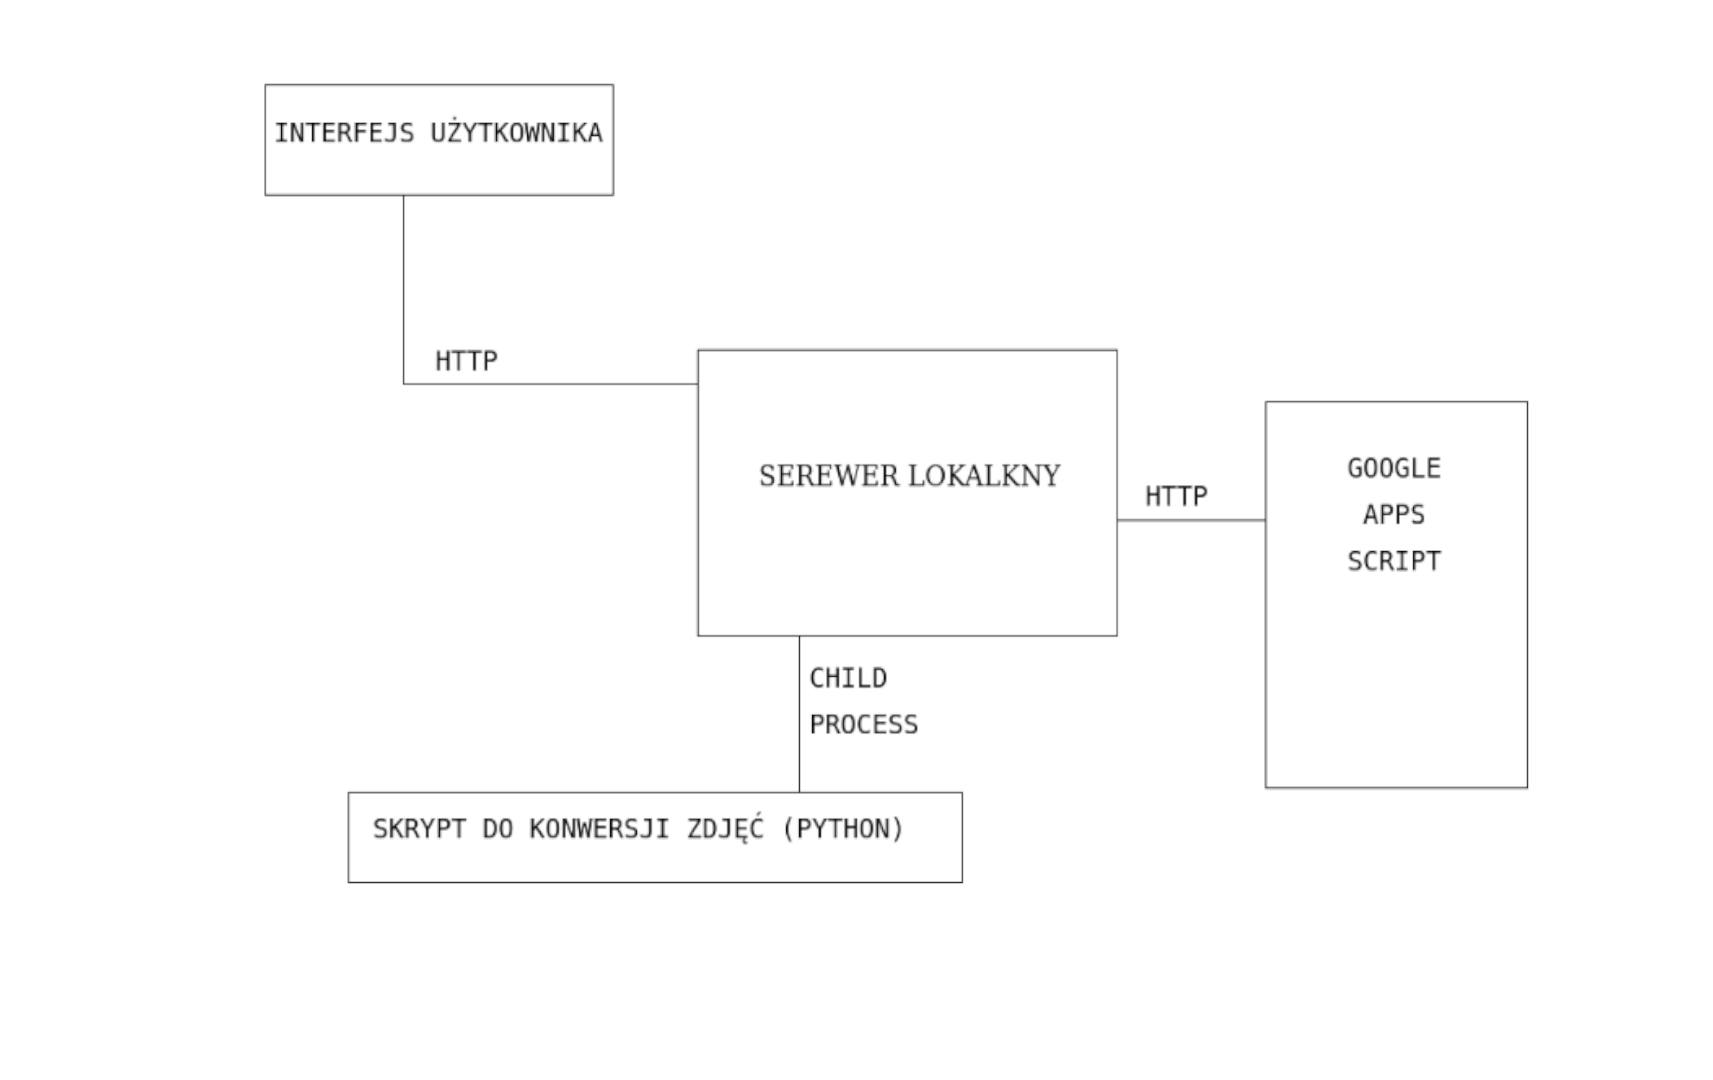
\includegraphics{schemat.png}
  \caption{Schemat połączeń}
  \label{fig:1}
\end{figure}

\section{Google Apps Script}
Nabudowywanie na gotowym narzędziu wymaga dostępu do niego. Google udostępnia API operujące na całym szeregu klas i metod oferowanych usług. Kod przypisany jest do danego konta Google, możliwe jest ustawienie parametrów,  takich  jak: kto ma dostęp do nowotworzonej aplikacji internetowej (właściciel, zalogowany użytkownik danej organizacji, dowolny zalogowany użytkownik, każdy) pod czyim kontem jest ona uruchamiana (właściciela/współwłaściciela, czy też zalogowanego użytkownika). 

\paragraph{Framework}
Udostępnione API w pewnym stopniu wymusza na użytkownikach, aby kod wykonywany na infrastrukturze Google'a był napisany w JavaScripcie, we framework'u ,,Google Apps Script''. Program jest wykonywany po stronie serwera. Pozwala on na stosunkowo łatwe manipulowanie działaniem produktów Google takich jak formularze, arkusze, dysk i inne. 
\ind Framework powstał w 2009 roku, w JavaScript 1.6, jest jednak regularnie ulepszany.

\paragraph{Komunikacja}
 Apps Script udostępnia komunikację przez protokół HTTP - jeśli projekt zawiera funkcje doGet(e) / doPost(e) - odpowiednie żądania wykonują kod z ciała tych metod. Zwracane wartości prowadzą do przekierowań zapytań  - automatycznie tworzony jest nowy adres URL. Wysłanie żądania GET pozwala na dotarcie do potrzebnych danych. 
\paragraph{API}
Google Apps Script udostępnia szereg klas i metod związanych z poszczególnymi narzędziami. Szczegółowa dokumentacja narzędzia znajduje się tutaj: Forms Service \cite{FormsService}.
 Główna klasa - FormApp - jest odpowiedzialna za zarządzanie formularzami - m.in. tworzenie nowych. Każdy typ pytania i element formularza ma odpowiednią klasę (jak np. CheckboxItem czy SectionHeaderItem). Poprzez klasę From  można zmieniać głowne ustawienia formularzy  - jak na przykład dodawanie właścicieli, tworzenie pytań, automatyczne ocenianie, manipulowanie tytułem, ustawienie, czy formularz jest ,,aktywny'' (czy przyjmuje odpowiedzi).
 
 
\section{Node.js}
Node.js jest środkowiskiem uruchomieniowym JavaScriptu - służącym do tworzenia aplikacji serwerowych. 
Praca wykorzystuje kilka bibliotek, przede wszystkim korzysta jednak z możliwości serwerowych Node.js. 
\paragraph{http}
Interfejs Node.js silnie związany z ,,sercem'' środowiska - udostępnia narzędzia do komunikacji poprzez protokół  HTTP zarówno ze strony serwerowej jak i klienckiej. W pracy w czystej formie wykorzystywany do wysyłania zapytań pomiędzy serwerem lokalnym a serwerem Google'a.
\newline Dokumentacja: http  \cite{https}
\paragraph{express}
,,Szybki (...), minimalistyczny framework webowy dla Node.js'' - narzędzie pozwala w przystępny sposób postawić serwer (korzysta z biblioteki http). Udostępnia cztery klasy:
\begin{itemize}
\item application - odpowiada aplikacji serwerowej,
\item  request - zarządza odwołaniami do serwera (głównie parametrami),
\item response - odpowiada za odpowiedzi serwera,
\item router - zajmuje się routingiem, może być używane jako oprogramowanie pośredniczące.
\end{itemize}
Trzon kodu narzędzia opiera się właśnie na serwerze express'owym.
\ind Dokumentacja znajduje się tutaj: expres.js \cite{express}.
\paragraph{cors}
Node.js'owy moduł pozwalający na odpowiednie ustawienia CORS (Cross-Origin Request Sharing) w rozwiązaniach typu express. CORS jest metodą rozwiązania problemów z domyślnymi ustawieniami związanymi z bezpieczeństwem. Standardowo dane z jednej strony mogą być pobierane z poziomu drugiej strony gdy obie strony są z tego samego źródła (ten sam schemat Url, host oraz port). CORS pozwala na uniknięcie tej konieczności.
\ind Github modułu: cors \cite{cors}
\paragraph{child\_process}
Moduł Node.js'owy pozwalający na uruchamianie podprocesów. W przypadku omawianego kodu, umożliwa uruchamianie skryptów napisanych  w Pythonie z poziomu kodu Node.js'owego.
\ind Dokumentacja znajduje się tutaj: child\_process \cite{childprocess}
\paragraph{jsonschema}
\ind Nowy (zaledwie dziesięciomięczny, wciąż w wersji Beta) moduł pozwalający na walidację formatu json zgodnie z podanym schematem.
\ind Oficjalna strona: jsonschema \cite{jsonschema}

\section{Python}
Rozwiązania pythonowe zostały wykorzystane w celu konwersji wstawek matematycznych (\LaTeX{}) do zdjęć. Poniżej krótki opis wykorzystanych bibliotek.
\paragraph{tex2pix} Biblioteka pozwalająca na konwertowanie formatu .tex do różnych formatów zdjęciowych. Metoda konwertująca format .tex na format .png zaczyna od konwersji .tex do .pdf, stąd w pracy używana jest konwersja do pdf z tej biblioteki, a dalsze manipulowanie formatem używa innych - subiektywnie prostszych w użytkowaniu - bibliotek. 
\ind Oficjalna strona: tex2pix \cite{tex2pix}.

\paragraph{pdf2image} Biblioteka  umożliwiająca konwersję formatu pdf do formatów zdjęciowych.
\ind Oficjalna strona: pdf2image \cite{pdf2image}.
\paragraph{opencv} Biblioteka pozwalająca na manipulację obrazami. Udostępnia znacznie więcej możliwości niż te użyte w pracy. W szczególności pozwala na przycinanie obrazów względem ich kolorystyki - co pozwala na automatyczne przycięcie strony pdf do rozmiarów napisanego na niej tekstu. Więcej informacji na temat biblioteki: opencv \cite{opencv}
\paragraph{base64} Biblioteka pozwala na konwersję obrazu do formatu Base64 - używanego w pracy do przesyłu obrazów pomiędzy serwerami node'owym a google'owym. 

\section{Bootstrap}  
Popularna biblioteka CSS, ułatwiająca budowanie interfejsów graficznych stron internetowych pisanych w HTML. Oficjalna strona bootstrap \cite{bootstrap}.





\chapter{Techniczny opis programu}
Narzędzie składa się z trzech głównych części:
\begin{itemize}
\item interfejsu użytkownika napisanego przy użyciu frameworku css'owego ,,Bootstrap'',
\item aplikacji internetowej, napisanej we frameworku Google Apps Script po stronie Google'a, pod prywatnym kontem e-mailowym, 
\item serwera napisanego w Node.js. Serwer jest uruchamiany lokalnie na urządzeniu użytkownika, komunikuje się z aplikacją internetową oraz interfejsem użytkownika.

\end{itemize}
Poza tym lokalny serwer wykorzystuje kilka bibliotek JavaScriptowych oraz Pythonowych do dodatkowych obliczeń. Schemat połączeń w projekcie:
\\tu będzie schemat narysowany\\%TODO
\section{Interfejs użytkownika}%TODO napisać o json sxhema i zlinkować następny rozdział (instrukcja, schemat
Na interfejs użytkownika składają się trzy pliki: \textit{strona.html}, \textit{memoryFile.js} oraz \textit{htmlCode.js} - pierwszy z nich koduje część wizualną, drugi dane na temat formularzy, trzeci jest odpowiedzialny za zachowanie poszczególnych elementów, w tym za komunikację z serwerem. 
\ind Elementami interfejsu są:
\begin{itemize}
\item pole do wgrywania plików, przyjmujące formaty .json oraz .txt. Zawartość powinna spełniać wymagania opisane w instrukcji w podrozdziale 4.2, %TODO link zrobić.
\item przycisk wgrywający plik - ,,generate form'' wywołuje metodę getFile,
\item listę formularzy, w której poprzez kliknięcie można wybrać formularz,
\item kilka przycisków powiązanych z metodą getInfo().
\end{itemize}
\ind Plik \textit{memoryFile.js} jest modyfikowany przez serwer lokalny i służy do zapamiętywania formularzy utworonych przez aplikację. Jako kod zawiera on wyłącznie deklarację stałej ,,memory'', będącej obiektem JSON następującej budowy:
\begin{lstlisting}[language=json,firstnumber=1]
{"forms":
    [{"id": "string",
      "date": "string",
      "name": "string"}
    ]
}
\end{lstlisting}
Wartość ,,id'' jest generowana przez usługę Google'a przy tworzeniu formularza, ,,date'' to data utworzenia formularza (rok-miesiąc-dzień), ,,name'' odpowiada tytułowi.
\ind Wartość ,,selectedForm'' z pliku \textit{htmlCode.js} odpowiada identyfikatorowi formjlarza obecnie podświetlonego na niebiesko na liście formularzy. Metody zaimplementowane w \textit{htmlCode.js}:
\begin{itemize}
\item changeLocation(newLocation) - pozwala na zmianę wyświetlanego adresu,
\item makeHttpRequest(Url, callback) - wysyła rządanie GET do lokalnego serwera (adres URL zależny jest od rodzaju przeprowadzanej akcji), w przypadku pozytywnej odpowiedzi (HTTP status 200) wywołuje metodę callback,
\item getInfo(action) - metoda przypisana większości przycisków interfejsu, jest odpowiedzialna za odpowiednie wywołanie makeHttpRequest,
\item getFile() - funkcja przypisana do przycisku ,,Generate form'', wczytuje wgrany plik, sprawdza, czy jest on poprawnym JSONem i wywołuje makeHttpRequest z odpowiednimi argumentami.
\item assign(id) - metoda przypisana do elementów listy formularzy, ustawia wartość ,,selectedForm'' przy każdej zmianie wybranego z listy formularza,
\item generateList() - tworzy listę formularzy na podstawie \textit{memoryFile.js}, jest uruchamiana przy ładowaniu strony.
\end{itemize}

\section{Google Apps Script}
Aplikacja internetowa stanowi rozwiązanie serwerowe, pozwalające na komunikację poprzez HTTP. Odwołać do niej może się każdy użytkownik znający adres url aplikacji, kod wykonywany jest pod kontem Google właściciela aplikacji (w chwili obecnej aplikacja jest utworzona pod prywatnym kontem Google).

\ind Po stronie Google'a znajdują się dwa pliki: \textit{communication.gs} oraz \textit{createFrom.gs}, odpowiadające kolejno za komunikację po HTTP oraz za zarządzanie tworzeniem formularzy. 
\subsection{HTTP}
Plik \textit{communication.gs} zawiera implementację metod doPost(e)oraz doGet(e). Framework zapewnia, że są one wykonywane, gdy do aplikacji przyjdą zapytania HTTP (odpowiednio POST i GET). Do parametrów funkcji są przekazywane treści zapytań.
\ind Metoda doGet(e) jest wykorzystywana do zapytań dotyczących tego, czy dany formularz przyjmuje przesyłane odpowiedzi oraz do uzyskiwania informacji na temat adresów URL danego formularza.  Poprawne zapytanie powinno zawierać dwie wartości:
\begin{itemize}
\item formId - identyfikator formularza przypisywany automatycznie w momencie tworzenia,
\item action - pole tekstowe mówiące o tym, co autor zapytania chce zrobić. Obsługiwane wartości:
\begin{itemize}
\item \textit{isActive} zwraca wiadomość tekstową informującą o tym, czy formularz przyjmuje odpowiedzi,
\item \textit{activate} aktywuje formularz (po wykonaniu tej częsci formularz przyjmuje odpowiedzi),
\item \textit{deactivate} dezaktywuje formularz,
\item \textit{publisherUrl} zwraca adres url formularza dla respondentów,
\item \textit{editorUrl} zwraca adres url do edycji formularza,
\item \textit{delete}.
\end{itemize}
\end{itemize}
Z braku udostępnionej metody usuwającej rządany formularz - zapytanie o usunięcie formularza dezaktywuje go. 
\ind Metoda doPost(e) odpowiada  za tworzenie nowych formularzy. Przesyłana zawartość zawiera zakodowany w formacie JSON formularz, wstępnie przetworzony przez lokalny serwer (zamiana pytań z wstawkami \LaTeX{}'owymi na zdjęcia w formacie base64). Ta metoda uruchamia funkcję \textit{createFromJSON} z pliku \textit{createForm.gs}.
\subsection{Zarządzanie formularzami}
Plik \textit{createForm.gs} zawiera kilka metod służących do tworzenia konkrentych rodzajów pytań:
\begin{itemize} %TODO rodzaje pytań
\item checkBox - 
\end{itemize}
Pytania ze wstawkami \LaTeX{}'owymi są w formie zdjęć, nie posiadają możliwych odpowiedzi - tuż pod nimi tworzy się pytanie bez treści zawierające możliwe odpowiedzi. W praktyce wygląda to w następujący sposób: (TU BĘDZIE ZDJĘCIE);
%TODO wstawić fotę
Takie rozwiązanie wynika z ograniczeń  API formularzy, które nie udostępnia metod wprowadzenia zdjęć do popularnych typów pytań - jest to znany problem, zgłaszany \href{https://issuetracker.google.com/issues/36765518?pli=1}{tutaj}. Metoda \textit{image} tworzy pole zdjęciowe w formularzu. 
Funkcja \textit{setFromFeatures} modyfikuje ustawienia formularza - chodzi tu o zapamiętywanie adresów mailowych użytkowników przesyłających odpowiedzi, limit odpowiedzi na użytkownika, ustawienie współwłaściciela formularza oraz wartości, czy formularz powinien być oceniany automatycznie.
\ind Główną funkcją w pliku jet \textit{createFromJSON}, która generuje formularz poprzez wywoływanie odpowiednich metod z wymienionych wyżej. Właścicielem formularza jest właściciel aplikacji internetowej (użytkownik Google, pod którego  kontem tworzone są formularze). Takie rozwiązanie pozwala na uniknięcie potrzeby autoryzacji przy każdym dostępie do aplikacji internetowej.
\section{Serwer Node.js'owy}
Serwer to prosta implementacja aplikacji we frameworku ,,express.js''. Po uruchomieniu nasłuchuje na porcie 3000 (co można zmienić w pliku \textit{server.js}, linia 3). Możliwe są trzy odwołania do serwera:
\begin{itemize}
\item uploadJsonFile
\item createForm
\item getInfo
\end{itemize}
Aplikacja korzysta z bibliotek ,,express'', ,,cors'', ,,fs'', ,,https'', ,,jsonschema'', ,,child\_process''  oraz skryptów \textit{jsonValidator.js} oraz \textit{tex2png.js} i \textit{text2png.py}.
Zaimplementowana metoda \textit{makeRequest(options, data)} służy do komunikacji z serwerem po stronie Google'a.
\ind Zasady działania poszczególnych fragmentów są opisane w odpowiednich podrozdziałach.
\subsection{Komunikacja międzyserwerowa}
Za komunikację pomiędzy serwerami odpowiedzialna jest metoda makeRequest(options, data) korzystająca z Node.js'owej biblioteki ,,https''. Zasada działania biblioteki jest następująca - https request przyjmuje dwa argumenty: pierwszy (options) deklaruje szereg parametrów ( adres URL zapytania, typ metody, zawartość, nagłówki zapytania itp.), drugi jest metodą wywoływaną na wartości zwracanej przez zapytanie. 
\ind Funkcja makeRequest(options, data) jako argumenty przyjmuje klasę options (zdefiniowaną w bibliotece https) oraz dane do przesłania. Zwraca konstrukcję Promise pozwalającą na szeregowanie kolejnych zapytań. Wewnątrz metody przechwytującej odpowiedź obsługiwane jest przekierowanie zapytania (wysyłane z każdą odpowiedzią Google'a zawierającą zawartość) - czyli wysyłane kolejne zapytanie do nowego adresu.
\subsection{Ścieżki serwera}
Poniżej przedstawiono obsługiwne ścieżki serwera wraz z opisem ich działania.
\paragraph{uploadJsonFile} Ścieżka pozwala na wgranie na serwer zakodowanego formularza i wstępne przetworzenie go. Ścieżka wywoływana jest z metody getFile() (patrz interfejs użytkownika, rozdział 3.1). Na początku kontrolowana jest zgodność kodowania ze schematem (plik \textit{jsonValidator}). Jeśli podany plik jest zgodny, przeprowadzana jest konwersja \LaTeX{}'a do zdjęć (plik \textit{tex2png.js}). Po tym etapie informacja o zgodności jest zwracana do interfejsu.
\paragraph{createForm} Jeśli interfejs otrzyma informację o zgodności wgranego JSONa ze schematem, wywołuje zapytanie do serwera na ścieżce createForm. W tym miejscu dla pytań z wartością ,,tex''=true serwer podmienia wartości ,,text'' pytań na kodowanie zdjęć w base64. Następnie wysyłane jest zapytanie POST do serwera po stronie Google'a z zakodowanym formularzem. Jeśli nie będzie błędów - zwrócona odpowiedź będzie zawierała identyfikator nowego formularza. W tym miejscu następuje również modyfikacja pliku \textit{memoryFile.js} - dodawany jest nowy element tabeli- data jest pobierana z klasy ,,Date'', nazwa z pola ,,title'' z kodowania formularza. Na koniec zwracana jest informacja do intefejsu.
\paragraph{getInfo} Za pomocą tej ścieżki  przekazywana jest komunikacja dotycząca istniejących formularz pomiędzy interfacem a serwerem Google'owym. Jest to też miejsce modyfikacji pliku \textit{memoryFile.js} - dla żądania ,,delete'' usuwany jest wpis dotyczący danego formularza.
\subsection{JSON validation} Plik zawiera deklarację schematu JSON (patrz: instrukcja, rozdział 4.2). Za pomocą biblioteki jsonschema wykonywana jest walidacja zawartości przesłanego pliku.
\subsection{Plik tex2png.js} Zadaniem tego modułu jest uruchomienie nowych procesów (child\_process.spawn)  - skrypt \textit{tex2png.py} w Pythonie zajmuje się konwersją tekstu na zdjęcia odpowiednich rozmiarów.
\section{Konwersja wstawek z\LaTeX{}'a}
Niniejsza część korzysta z podstawowej bibioteki \LaTeX{}'a, szablon tworzonych zdjeć stanowi plik \textit{texTemplate.tex}. Wszystkie tworzone pliki znajdują się w folderze \textit{pictures}.
\ind Decyzja o napisaniu tej części w Pythonie powstała stosunkowo późno. Powodem jest biblioteka openCV - udostępniająca zaawansowane metody obliczeniowe w przystępny sposób. Skrypt działa następująco:
\begin{itemize}
\item Wczytywany jest szablon w \LaTeX{}'u i w odpowiednie miejsce wstawiany jest tekst z pytania (oznaczonego tex=true) - warto wspomnieć, że treść pytania jest otoczona ramką.
\item Za pomocą biblioteki tex2pix plik .tex jest konwertowany do formatu pdf.
\item Biblioteka pdf2image konwertuje pdf'a do png.
\item Biblioteka openCV pozwala na ,,wycięcie'' ze zdjęcia wyłącznie obszaru otoczonego ramką (jako jedyny zawiera kolory).
\item ,,Ramka'' jest zapisywana jako png.
\item Przy użyciu biblioteki base64 końcowe zdjecie jest konwertowane do formatu base64 i zapisywane do pliku.
\item Pośrednie stadia konwersji są usuwane z folderu.
\end{itemize}
\subsection{Alternatywne rozwiązanie}%o tym czemu nie mathjax
Wydaje się naturalne, aby do problemu parsowania symboli matematycznych użyć gotowego silnika (opartego np. na Markdown'ie lub \LaTeX{}'u). Takim silnikiem jest na przykład MathJax. Udostępnia bogate API, integrację Webową. Doskonale współpracuje z JavaScriptem. Narzędzie jest jednak stosunkowo świeże, a główną komplikacją jest to, że zwracany wynik jest w HTMLu - co wymagałoby dodatkowej konwersji. Nie wykluczone jednak, że istnieje znacząco prostsze rozwiązanie - korzystające właśnie z takiego silnika.
\section{Skrypty instalujący i uruchamiający}
Instalacja oparta jest na npm (dla Node.js) i pip (Python) - skrypt \textit{install.sh} instaluje wymagane biblioteki przy pomocy tychże narzędzi.
\ind  Uruchomienie programu wymaga uruchomienia dwóch części - serwera lokalnego oraz interfejsu - ten drugi wymaga przegląarki internetowej. Skrypt \textit{run.sh} wypisuje ścieżkę pliku stanowiącego interfejs z prośbą o otwarcie go w przeglądarce i uruchamia serwer lokalny.












\chapter{Instrukcja użytkownika}
\section{Początki pracy  z narzędziem}
Wtyczka pozwala na wygenerowanie formularza Google Forms z pliku kodującego w formacie JSON, automatyczne definiowanie jego treści na podstawie wstawek w \LaTeX{}'u oraz zarządzanie informacjami o tym, czy dany formularz przyjmuje przesyłane odpowiedzi. Na początek należy jednak pobrać i zainstalować zależności wykorzystywane przez narzędzie.
\subsection{Instalacja}
Na początku należy sklonować \href{https://github.com/agnpawicka/pracaInzynierska/}{repozytorium projektu} --- github.com/agnpawicka /pracaInzynierska.
\ind Następnie wejść w folder \textbf{source} i uruchomić plik o nazwie ,,install.sh''. Pozwoli to na zainstalowanie potrzebnych bibliotek.
\subsection{Praca z wtyczką}
Aby włączyć narzędzie należy uruchomić plik o nazwie ,,run.sh''. Uruchomi on lokalny serwer Node.js-owy oraz stronę internetową z interfejsem użytkownika.
\section{Schemat pliku kodującego (JSON)}
Poniżej znajduje się rozpisany schemat kodowania: 
\begin{figure}[H]
\begin{lstlisting}[language=json,firstnumber=1]
{"title": "string",
 "email": "string",
 "check": "boolean",
 "questions": {[{"type": "string", 
                 "text": "string",
                 "tex" : "boolean",
                 "answers": [{"answer" : "string",
                             "correct" : "boolean"}],
                 "points": "number"}]}
}

\end{lstlisting}
\end{figure}
Jest to opis tych wartości, które mogą być użyte -- nie wszystkie są jednak  wymagane. Poniżej znajduje się szczegółowy opis pól i wartości:
\begin{itemize}
\item{title} -- wartość tekstowa, odpowiada nagłówkowi formularza -  \textbf{pole wymagane},
\item{email} -- adres e-mail edytora formularza (konieczne konto google) -- \textbf{pole opcjonalne},
\item{check} -- wartość boolowska mówiąca o tym, czy formularz ma udostępniać opcję automatycznego oceniania. Domyślna wartość to \textbf{false}. W przypadku ustawienia wartości na \textbf{true} należy się upewnić, że przy każdym pytaniu są poprawnie ustalone wartości ,,correct'' oraz ,,points'' -- \textbf{pole opcjonalne},
\item{questions} -- tablica, której każde pole zawiera informacje dotyczące jednego pytania -- \textbf{pole wymagane}. Poniżej znajdują się wartości kodujące pojedyncze pytanie:
\begin{itemize}
\item{type} -- pole tekstowe dotyczące typu kodowanego pytania. Dopuszczalne wartości:
\begin{itemize}
\item ,,checkBox'' -- pytanie zamknięte wielokrotnego wyboru,
\item ,,grid'' -- pytanie typu ,,prawda/fałsz'',
\item ,,list'' -- zamknięte jednokrotnego wyboru,
\item ,,text'' -- otwarte.
\end{itemize}
 \textbf{pole wymagane},
\item{text} -- zawiera treść pytania w formie tekstowej. Może zawierać wstawki z \LaTeX{}'a. Należy jednak pamiętać, że JavaScript traktuje symbol ,,$\backslash$'' jako specjalny -- wszystkie wystąpienia ,,$\backslash$'' należy więc zastąpić ,,$\backslash\backslash$'' -- \textbf{pole wymagane},
\item{tex} -- wartość boolowska, jeśli \textbf{true} treść pytania (text) będzie konwertowana do obrazu z zachowaniem konwersji symboli matematycznych i innych wstawek z \LaTeX{}'a z biblioteki standardowej, \textbf{pole wymagane},
\item{answers} -- tablica, każde pole zawiera jedną z możliwych odpowiedzi w następującej formie:
\begin{itemize}
\item answer -- pole tekstowe, treść danej odpowiedzi
\item correct -- wartość boolowska wskazująca czy dana odpowiedź jest prawidłowa. Domyślna wartość: false.
\end{itemize} 
-\textbf{pole opcjonalne}
\item{points} -- wartość numeryczna, odpowiada liczbie punktów przyznawanej za poprawą odpowiedź na pytanie (dotyczy wyłącznie oceniania automatycznego) -- \textbf{pole opcjonalne}
\end{itemize}
\end{itemize}









\section{Obsługa narzędzia}
Po uruchomieniu użytkownik widzi stronę w przeglądarce, jak na zdjęciu poniżej:
\begin{figure}[H]
  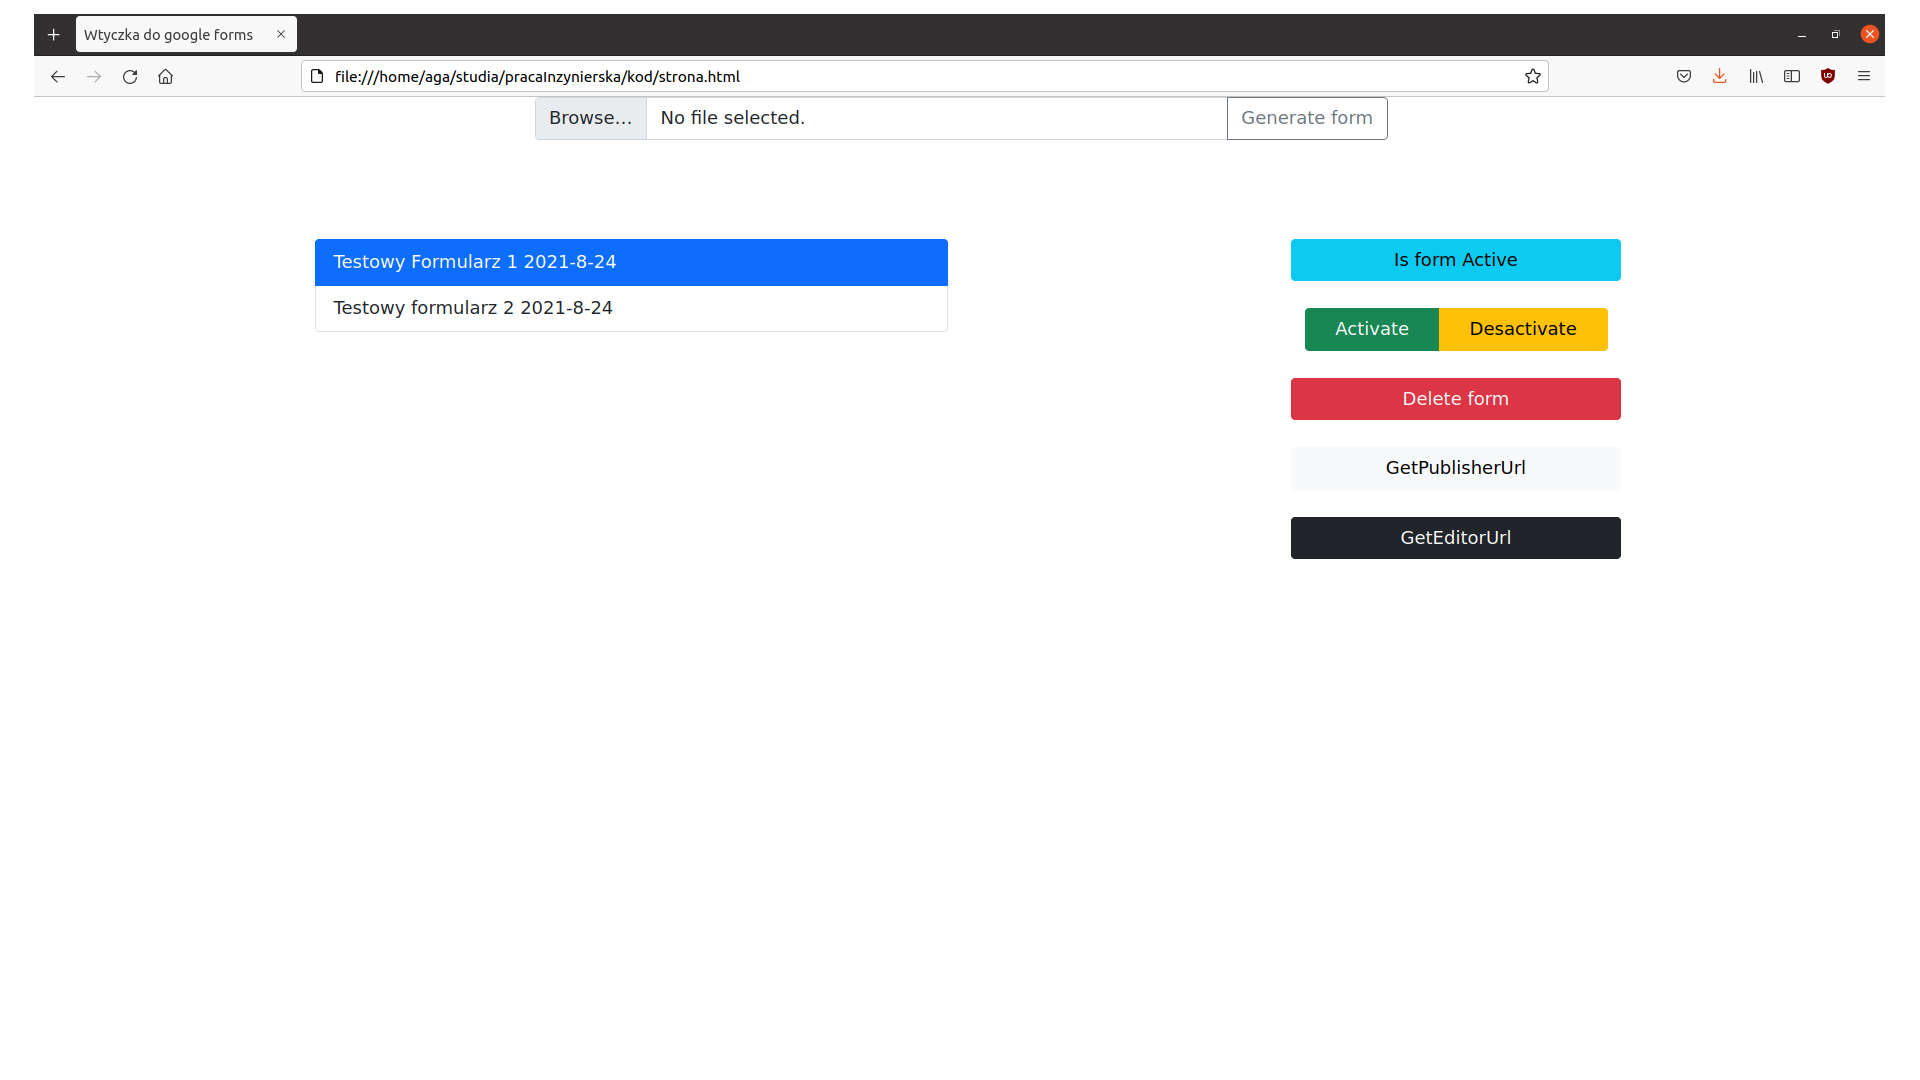
\includegraphics[scale=0.75]{strona.png}
  \caption{Interfejs aplikacji}
  \label{fig:1}
\end{figure}
\\Widoczne u góry pole do wgrywania plików przyjmuje formaty .txt oraz .json. W pliku powinien znajdować się zakodowany formularz (podrozdział 4.2. Schemat pliku kodującego (JSON)).
\\Poniżej  po lewej stronie znajduje się lista utworzonych już formularzy, po prawej znajdują się przyciski służące do operowania na już istniejących formularzach.
\\Przycisk ,,Generate form'' wgrywa podany plik i  wykonuje na nim kolejne operacje. Poprawne wykonanie powinno przechodzić przez kolejne etapy:
\begin{itemize}
\item Sprawdzany jest format  pliku. Jeśli zawartość jest obiektem typu JSON, dane przekazywane są do lokalnego serwera, w przeciwnym przypadku strona wyświetli alert informujący o niepoprawnym formacie.
\item Serwer lokalny sprawdza zgodność pliku ze schematem (JSON schema). Po tym etapie poniżej pola do wgrywania plików powinna pojawić się jedna z poniższych informacji:
\begin{itemize}
\item Validation succeded
\item Wrong JSON format
\end{itemize}
\item Jeśli plik JSON jest zgodny ze schematem, następuje konwersja pytań zakodowanych jako ,,tex'' na format graficzny. 
\item Po zakończonej konwersji, z lokalnego serwera wysyłany jest POST request do serwera po stronie Google, gdzie odbywa się konwersja pliku na formularz. Zdalny serwer odsyła informację po zakończonej pracy do serwera lokalnego.
\item Lokalny serwer dodaje nowy formularz do listy.
\item Wyświetla się komunikat \textbf{New form has been created. Please reload the page} z prośbą o odświeżenie strony.
\end{itemize}
\ind Zachowania poszczególnych przycisków  -- za wyjątkiem ,,Generate Form'' -- dotyczą zawsze wybranego formularza z listy (podświetlonego w danym momencie na niebiesko). Aby wybrać formularz należy kliknąć na niego w liście formularzy. 
\ind Widoczne w interfejsie przyciski mają następujące funkcje:
\paragraph{Is Form Active} zwraca wartość \textbf{Form is active} jeśli formularz przyjmuje odpowiedzi oraz \textbf{Form is inactive} w przeciwnym przypadku.
\paragraph{Activate} wysyła do serwera po stronie Google'a zapytanie, jeśli aktywacja formularza przebiegła pomyślnie, zwracana jest wiadomość \textbf{Form activated}.
\paragraph{Deactivate} wysyła do serwera po stronie Google'a zapytanie, jeśli dezaktywacja formularza przebiegła pomyślnie, zwracana jest wiadomość \textbf{Form deactivated}.
\paragraph{Delete Form} wysyła do serwera po stronie Google'a zapytanie o dezaktywację formularza, następnie usuwa z pliku z danymi o formularzach wpis dotyczący wybranego formularza oraz w komunikacie \textbf{Form deactivated, please reload page.} prosi o odświeżenie strony.
\paragraph{Get Publisher Url} wysyła do serwera po stronie Google'a zapytanie o adres url dla respondentów wybranego formularza. W komunikacie pojawia się odpowiedni link.
\paragraph{Get Editor Url} wysyła do serwera po stronie Google'a zapytanie o adres url dla edytorów wybranego formularza. W komunikacie pojawia się odpowiedni link.



\chapter{Podsumowanie}%problemy i rozwój o konkluzje

\section{Wnioski}
Celem pracy była implementacja narzędzia pozwalającego na uproszczenie przeprowadzania testów i ankiet online w oparciu o istniejące już rozwiązanie -- Google Forms.  Efektem jest program, ułatwiający pracę z formularzami Google'a poprzez umożliwienie automatycznego generowania pytań oraz konwersję symboli matematycznych.  Możliwe jest jednak dalsze rozwijanie narzędzia. 

\section{Rozwój}
Możliwych rozszerzeń jest wiele -- niniejszy rozdział opisuje kilka z nich.
\paragraph{Zarządzanie przesłanymi odpowiedziami} -- Google Apps Script udostępnia klasę ItemResponse -- odpowiedzialną za zarządzanie odpowiedziami respondentów. Możliwe jest przechwytywanie odpowiedzi, oceny (wystawionej automatycznie, jeśli tak ustawiono), pytania, do którego jest odpowiedz (jako klasy, a wiec razem z możliwymi odpowiedziami, punktami, treścią) a także ustawienie komentarza. Dalej: możliwe jest przetwarzanie pozyskanych danych i ocenianie testów przez zewnętrzny program na niestandardowych zasadach (jak na przykład wykładnicza skala punktowa w zależności od liczby poprawnych odpowiedzi).
\paragraph{Możliwość ustawiania losowej kolejności pytań} -- choć w teorii ten problem jest rozwiązany przez udostępnione API, w praktyce pojawia się problem. Jak wspomniano wyżej -- API formularzy nie udostępnia metod wprowadzenia zdjęć do popularnych typów pytań. Powoduje to konieczność utrzymywania dwóch formalnie osobnych pytań (w praktyce pytania-zdjęcia i odpowiedzi) w jednym miejscu w formularzu.
\paragraph{Ustawianie czasu rozpoczęcia oraz zakończenia testu} -- aby mogło się to odbywać automatycznie, potrzebne jest urządzenie, które będzie regularnie i w krótkich odstępach czasowych sprawdzało, czy należy już wysłać odpowiednie zapytanie do zaimplementowanej aplikacji, czy jeszcze nie. Może się to wykonywać po stronie serwera lokalnego lub w samej aplikacji internetowej -- po stronie Google'a. Zaimplementowany serwer nie uwzględnia jednak tej możliwości ze względu na konieczność ciągłego trwania w stanie uruchomionym. 



%%%%% BIBLIOGRAFIA


\bibliographystyle{unsrt} %{abbrv} % unsrt sortuje według kolejności wystąpień
\bibliography{bibliography}

\appendix

\end{document}
